\chapter{Preliminares}

En este capítulo se presentan conceptos fundamentales para la comprensión de esta tesis.
Se comienza con una descripción del funcionamiento de Internet, su estructura y componentes fundamentales. Luego, se explica el protocolo de enrutamiento BGP, a través del cual se obtuvo la información de ruteo para construir el grafo.
Finalmente, se provee una explicación del funcionamiento de las Redes Neuronales de Grafos (GNN), herramienta que se utilizó para la tarea de inferencia de relaciones económicas entre Sistemas Autónomos.\\

\section{Internet} \label{internet_section}

El \textbf{Internet} es una \textbf{red global de redes} que interconecta miles de dispositivos en todo el mundo que proporcionan servicios a aplicaciones distribuidas~\cite{Computer-Networking}. Entre estos dispositivos se encuentran computadoras, teléfonos celulares, servidores de contenido y muchos otros.\\

Cuando un dispositivo final intenta establecer una conexión a través de Internet, los datos a enviar son encapsulados en paquetes con cabeceras que contienen la información necesaria para llegar al dispositivo final.
En algunos casos los datos pueden ser divididos en diferentes paquetes y ser enviados por distintas rutas hasta llegar al dispositivo final, donde son reensamblados. 
El recorrido que sigue un paquete desde su origen hasta su destino a través de distintos routers se conoce como ruta. \\


Los sistemas finales acceden a Internet por medio de proveedores de Internet (ISPs), los cuales, a su vez, son redes conformadas por routers y enlaces de comunicación. 
Estos ISPs de nivel inferior se conectan a ISPs de nivel superior, nacionales e internacionales como Level 3, Cogent, entre otros~\cite{ASRank-web}, que se encuentran en la cima de la jerarquía de Internet, al tener conexiones directas con el \textit{backbone} de Internet. En la Figura~\ref{fig:estructura_internet} podemos ver un un ejemplo del orden jerárquico del Internet explicado previamente. \\

\begin{figure}[h]
    \centering
    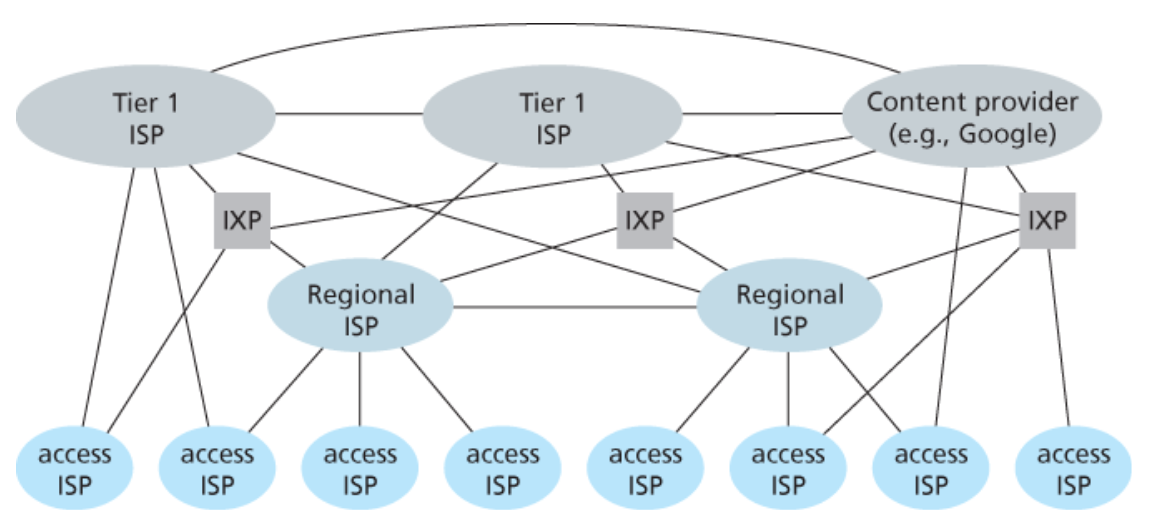
\includegraphics[width=0.7\textwidth]{img/internet/Estructura-Internet-ISP.png}
    \caption{Ejemplo de estructura jerárquica de Internet}
    \label{fig:estructura_internet}
\end{figure}



Así, estos proporcionan a los usuarios finales el acceso a proveedores de contenido (CDN, por sus siglas en inglés), sitios web y otros servicios, los cuales también están conectados a la infraestructura de Internet.\\

% Para el correcto funcionamiento de Internet existen diferentes protocolos, sin embargo, los dos más importantes corresponden al Protocolo de Control de Transmisión (TCP) y el Protocolo de Internet (IP),conocidos colectivamente como TCP/IP. El desarrollo de estos estandares los lleva acabo el Internet Engineering Task Force (IETF) \cite{IETF}, y los documentos se conocen como Requests for Comments (RFCs).

\section{Sistemas Autónomos} \label{sec:sistemas_autonomos}

En la estructura de Internet, un Sistema Autónomo (AS) consiste en un conjunto de routers y enlaces de comunicación que comparten una política de enrutamiento común. Estos son operados de forma independiente por organizaciones, como ISPs , universidades, empresas, entre otras.\\



\begin{figure}[h]
    \centering
    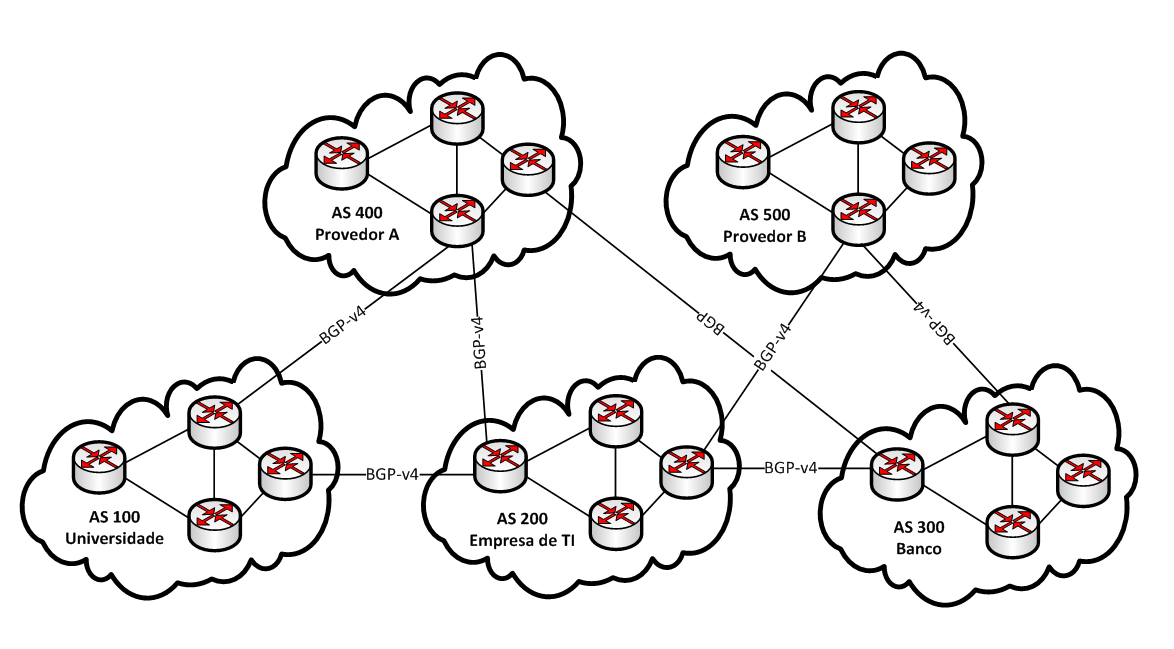
\includegraphics[width=0.5\textwidth]{img/internet/topologiaBGP.png}
    \caption{Ejemplo de topología a nivel de Sistemas Autónomos.}
    \label{fig:topologia-ASes}
\end{figure}

Los ASes utilizan el protocolo BGP para intercambiar información de enrutamiento entre ellos y así lograr una conexión global entre ASes y, por ende, en Internet. Las conexiones entre los Ases pueden ser de tipo cliente-proveedor, peer-to-peer o sibling-to-sibling, pero están influenciadas por acuerdos comerciales. Bajo estos acuerdos, podemos crear un grafo de la infraestructura de Internet, donde los nodos son los ASes y las aristas son las conexiones entre ellos. Cabe destacar que, en este caso, una conexión no implica necesariamente el intercambio de tráfico entre los ASes conectados, ya que el enrutamiento está controlado por BGP, un protocolo de enrutamiento basado en políticas~\cite{InferringASRelatioships2001}.\\

En la Figura~\ref{fig:topologia-ASes} se observa una serie de Sistemas Autónomos: proveedores de servicios (AS 400 y AS 500), una universidad (AS 100), una empresa de TI (AS 200) y un banco (AS 300). Cada uno está compuesto por múltiples routers, donde únicamente los routers de borde de cada AS se conectan mediante sesiones BGP con otros Sistemas Autónomos.\\

Otro concepto importante para entender la estructura de Internet son los Internet Exchange Points (IXPs). Estos corresponden a puntos de interconexión, donde múltiples ASes se conectan, y establecen conexión con otros ASes sin necesidad de estar directamente conectados.

Más información sobre los Sistemas Autónomos y los IXPs puede encontrarse en los Anexos \ref{sec:sistemas_autonomos_section} y \ref{sec:ixp_section}, respectivamente.


\section{Ruteo}


Antes de introducir el protocolo BGP, debemos entender brevemente el \textbf{ruteo}.\\


El \textbf{ruteo} es el proceso mediante el cual se selecciona el camino que seguirá un paquete dentro de una red para llegar a su destino final. 
El camino que sigue un paquete se elige según la información de las \textbf{{tablas de enrutamiento} (\textbf{RIBs}) de los routers y la información contenida en los \textbf{encabezados de los paquetes}}, donde se indica el destino final.\\



Cuando un paquete llega a un \textbf{router}, se consulta en la \textbf{tabla de enrutamiento} la dirección final para obtener el próximo router o punto de red al cual se debe dirigir el paquete.\\



Por ejemplo, cuando un usuario accede a una página web desde su hogar, los paquetes viajan desde el servidor que aloja la página web hasta el router de su casa. 
Este router luego examina el encabezado del paquete para identificar el destino final, consulta su tabla de enrutamiento y lo reenvía al siguiente punto de la red. 
Este nuevo router intermedio repite el proceso hasta que el paquete alcanza su destino final.\\



Existen dos tipos de enrutamiento: \textbf{estático} y \textbf{dinámico}. 
El enrutamiento \textbf{estático} implica el uso de tablas fijas, las cuales deben ser modificadas manualmente para cambiar su configuración. 
Por otro lado, en el enrutamiento \textbf{dinámico}, los routers se encargan de actualizar las tablas de enrutamiento en tiempo real, ajustándolas según las condiciones de la red.\\
%Este proceso se lleva a cabo mediante los protocolos de enrutamiento.\\


Dicho esto, podemos representar el \textbf{grafo de Internet} como el grafo \textbf{$G = (N, E)$}, donde $N$ corresponde al conjunto de \textbf{ASes} y $E$ al conjunto de \textbf{aristas} entre estos, las cuales representan si un paquete en Internet puede ocupar dicho enlace para llegar de un punto a otro.

\section{Border Gateway Protocol (\textbf{BGP})}

Como se mencionó, existen dos tipos de ruteo: estático y dinámico. 
BGP~\cite{RFC-BGP} pertenece al tipo dinámico; este se encarga de analizar todas las posibles rutas a los diferentes destinos y seleccionar la mejor ruta. 
Luego, comparte esta información con sus ASes vecinos, quienes a su vez repiten el proceso. 
Así, cada Sistema Autónomo (AS) genera caminos hacia los distintos prefijos de Internet y, cuando ocurren cambios en la red, BGP también se encarga de actualizar las rutas mediante el intercambio de mensajes \textit{UPDATE}.\\


BGP comienza una vez que se ha establecido la conexión TCP entre los pares BGP, estos intercambian mensajes \textit{OPEN} para confirmar los parámetros de la sesión. Luego, envían un mensajes \textit{KEEPALIVE} para confirmar la conexión.\\

La información que se intercambia en primera instancia consiste en una porción de la tabla de información de BGP, llamada \textit{Adj-RIB-Out}, la cual está filtrada de acuerdo a las políticas locales de exportación hacia los diferentes ASes. A medida que esta tabla va cambiando, se envían actualizaciones incrementales mediante mensajes \textit{UPDATE}. \\
Además, para asegurar que la conexión sigue activa, los pares BGP intercambian cada cierto tiempo mensajes \textit{KEEPALIVE}.\\

En caso de que se detecte algún tipo de error durante la conexión, se envía un mensaje \textit{NOTIFICATION} el cual indica el tipo de error y tras su envío la conexión BGP se cierra y todas las rutas aprendidas en la sesión son eliminadas.\\

La Figura~\ref{fig:Funcionamiento-BGP} muestra cómo BGP propaga la información de ruteo entre distintos AS.
Cada sistema autónomo anuncia la dirección de destino a sus pares, en este caso específico el AS 64503 anuncia su dirección a sus pares $64502$ y $64504$, quienes a su vez anuncian la dirección a sus pares, modificando el \textit{AS\_PATH}  a medida que la información se propaga. Finalmente, el AS 64501 recibe estos anuncios y, basándose en la información acumulada, determina la mejor ruta para alcanzar la red del AS 64503.\\


\begin{figure}[H]
    \centering
    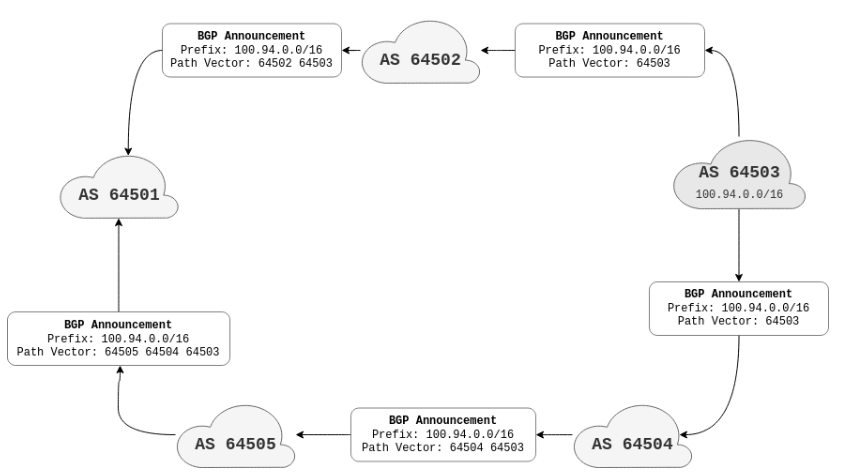
\includegraphics[width=0.7\textwidth]{img/internet/BGPFuncionamiento.png}
    \caption{Ejemplo de propagación de mensajes UPDATE. En este caso AS 6453 comienza anunciando su dirección a sus pares.}
    \label{fig:Funcionamiento-BGP}
\end{figure}


Más información sobre los tipos de mensajes del protocolo puede encontrarse en el Anexo \ref{sec:anexo_mensajes_bgp}.

\subsection{\textbf{BGP} Routing Information Base (RIB)}

Otro concepto importante son las tablas RIBs. A partir de las cuales se extrajo la información para construir el grafo de Internet y la arista que conectan a los ASes en este trabajo.\\

Cuando se utiliza BGP, los routers BGP reciben mensajes \textit{UPDATE} de sus vecinos, los cuales son analizados y filtrados según las políticas locales de ruteo del AS, para luego anunciar las rutas seleccionadas a sus vecinos. Para esto, BGP utiliza una base de datos denominada Routing Information Base (RIB), que se compone de tres partes:\\

\begin{itemize}
    \item \textbf{Adj-RIB-In:} Almacena la información de ruteo de los mensajes \textit{UPDATE} recibidos de los vecinos BGP.
    \item \textbf{Loc-RIB:} Contiene la información de ruteo local, es decir, las mejores rutas seleccionadas para cada dirección.
    \item \textbf{Adj-RIB-Out:} Guarda la información seleccionada por el router para ser anunciada a sus pares. Consiste en la información de \textit{Loc-RIBs} luego de ser aplicadas las políticas internas de ruteo. Esta es la información que se incluye en los mensajes \textit{UPDATE}.
\end{itemize}

El flujo de información en BGP y el proceso de toma de decisiones de rutas se realiza de la siguiente manera:
primero, se reciben los mensajes \textit{UPDATE} de los vecinos, los cuales se almacenan en la \textit{Adj-RIB-In}, una entrada por cada vecino. Luego, se evalúa el grado de preferencia de cada ruta almacenada en la \textit{Adj-RIB-In}. En base en esta evaluación, se seleccionan las mejores rutas para cada destino y se instalan en la \textit{Loc-RIB}. Finalmente, la información contenida en la \textit{Loc-RIB} se transfiere a la \textit{Adj-RIB-Out} para ser anunciada a los vecinos BGP, siguiendo las políticas de ruteo locales. Este flujo de información se conoce como el proceso de decisión BGP.\\

Es importante destacar que las bases de datos que almacenan la información de rutas BGP no son lo mismo que la tabla de ruteo de un router, que es la que el router utiliza para realizar el forwarding de los paquetes. Las rutas almacenadas en la RIB deben cumplir con ciertos criterios, definidos por el software o el proveedor del router, para ser agregadas a la tabla de ruteo.\\


\section{Redes Neuronales}

A continuación, se presenta una introducción básica a las Redes Neuronales, para luego pasar al funcionamiento y arquitecturas básicas  de las Redes Neuronales de Grafos, las cuales fueron utilizadas en el desarrollo de esta tesis.\\

Una Red Neuronal es un modelo computacional compuesto de neuronas (perceptrones), dispuestas en capas y conectadas entre sí con el fin de aprender patrones mediante el intercambio de información ponderada por pesos. Estos pesos se ajustan en base a los datos de entrada, asignando valores en función del reconocimiento de patrones, que permiten una salida esperada.\\


\begin{figure}[h]
    \centering
    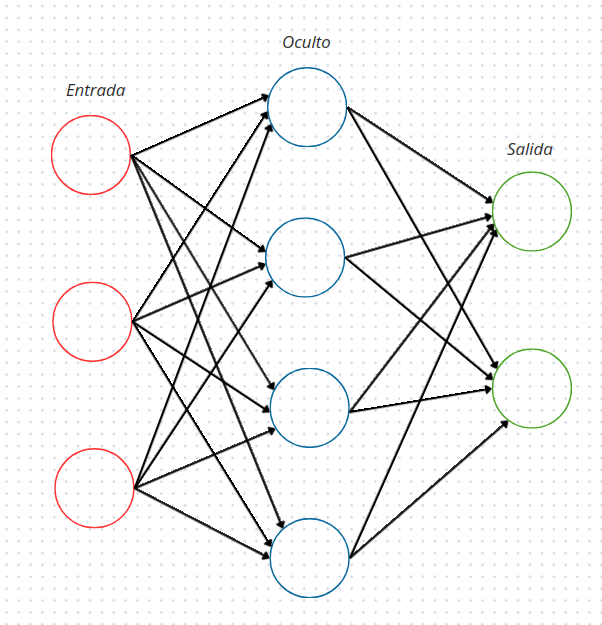
\includegraphics[width=5cm]{img/redesNeuronales/red_neuronal.png}
    \caption{Arquitectura básica de una Red Neuronal Fully Connected de una capa.}
    \label{fig:fully-connected}
\end{figure}


En una Red Neuronal, cada unidad toma entradas, las pondera por separado, suma los valores y pasa esta suma a través de una función para producir una salida, la cual es compartida con otras neuronas a las cuales está conectada.\\


El perceptrón, que funciona como una representación matemática de una unidad básica en la Red, realiza cálculos para determinar tendencias en los datos de entrada, asignándole diferentes pesos a cada valor de entrada en base a patrones entre los datos para realizar tareas específicas.\\


Un perceptrón está compuesto por cuatro elementos distintivos (Figura \ref{fig:perceptron}), i) los valores de entrada definidos como $x_i, x_{i+1} , ... , x_{n-1}, x_n$ donde cada $x_j$ corresponde a un vector de tamaño d, ii) los pesos definidos como  $w_j \in \mathbb{W}^{n \times d}$ donde $\mathbb{W}$ corresponde a la matriz de pesos los cuales son ajustados durante la etapa de entrenamiento de la Red, iii) la suma $z = \sum_{j=1}^{d} w_j x_j + b$ y iv) la función de activación, la cual establece un umbral de salida para evitar que los valores de salida se disparen. Esta función de activación permite incluir más capas y, por ende, mayor complejidad en las arquitecturas de redes que se construyan. Las funciones de activación tienen la capacidad de mejorar el aprendizaje de patrones en los datos~\cite{activation-function}.
Algunas de las funciones de activación comúnmente empleadas incluyen la Sigmoide, la Tangente Hiperbólica (tanh), la Rectified Linear Unit (ReLU) y la  Leaky ReLU.\\


\begin{figure}[h]
    \centering
    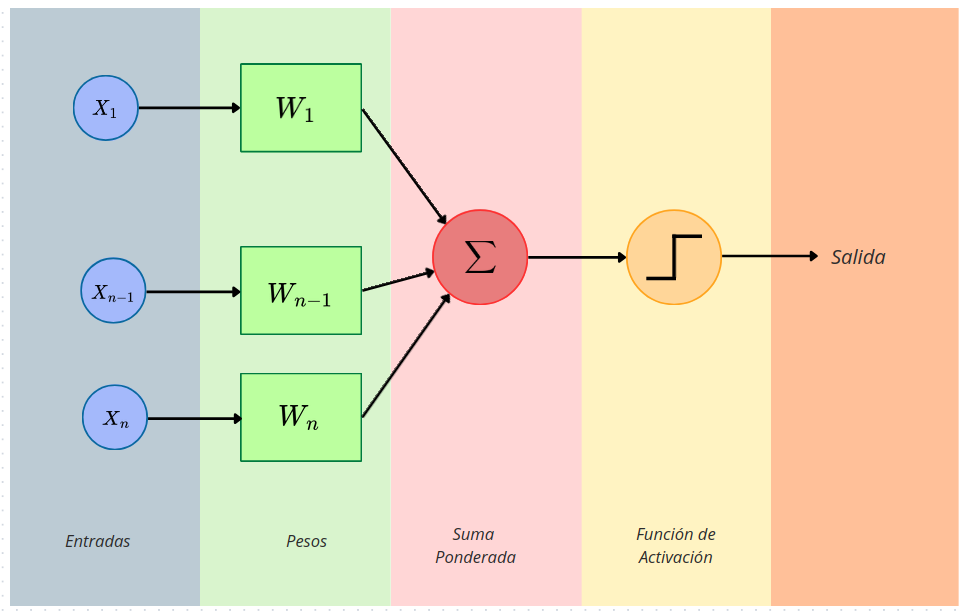
\includegraphics[width=10cm]{img/redesNeuronales/perceptron.png}
    \caption{ Estructura general de un perceptrón. }
    \label{fig:perceptron}
\end{figure}


La técnica comúnmente utilizada para el entrenamiento de Redes Neuronales es el \textit{backpropagation},
que tiene como objetivo ajustar los pesos de los parámetros de la Red para minimizar la función de pérdida~\cite{back-propagation}. Esta función cuantifica la diferencia entre las predicciones hechas y los valores reales. Una vez que se ha calculado la pérdida, el proceso de optimización se centra en modificar los pesos para mejorar la precisión general de la Red.\\

Durante el entrenamiento de las Redes Neuronales, se emplea el descenso de gradiente, un método que implica el cálculo de la derivada de la función de pérdida con respecto a los pesos de la Red. Este cálculo determina la dirección y magnitud en la que los parámetros de un modelo deben ser ajustados para minimizar la función de pérdida. Por ende, es fundamental que esta función sea continua y derivable.
En problemas de regresión, se suele utilizar funciones como el Mean Squared Error y Mean Absolute Error, mientras que en problemas de clasificación, destaca la Cross-Entropy Loss. \\


\section{Graph Neural Network (GNN)}

Las GNN son una arquitectura de redes neuronales especialmente diseñada para realizar predicciones basadas en datos representativos de grafos~\cite{scarselli_graph_2009}. A diferencia de las Redes Neuronales convencionales, las GNNs reciben datos en forma de tensores que pueden representar nodos, atributos de nodos, aristas y atributos de aristas.\\

% Existen diferenets enfoques, dependiendo de la tarea de aprendizaje que se quiere llevar a cabo, estos son:

% - Nivel de nodo: Incluye tareas como clasificación, regresión y clustering de nodos. Se realizan inferencias a partir de las conexiones con otros nodos. 


% - Nivel de  aristas: Se abordan tareas de clasificación y predicción de aristas. Por ejemplo, determinar la existencia de una relación entre dos nodos.

% - Nivel de grafo: Se encuentran tareas de clasificación, regresión y matching de grafos para las cuales el modelo debe ser capaz de aprender una representación para el grafo completo.


Las GNN tienen una serie de ventajas sobre las Redes Neuronales convencionales cuando se trabaja con datos de grafos. En contraste con los modelos tradicionales, las GNN aprovechan las relaciones entre las entidades que conforman los datos de entrada a el modelo. Estas relaciones pueden incluir aspectos como orden, jerarquía, dependencias o relaciones de otro tipo que son comunes en grafos y se representan a través de las aristas que conectan los nodos.\\

En cuanto a la adaptabilidad a variaciones en el tamaño de entrada, las Redes Neuronales convencionales requieren que los datos de entrada mantengan un mismo tamaño. Para ello, recurren a técnicas como padding o broadcast, los cuales no tienen efectos significativos en el desempeño de los modelos. Las GNNs, por su parte, ofrecen flexibilidad para adaptarse a distintos tamaños de entrada~\cite{GCN}.\\

Otro motivo para optar por GNNs es su capacidad para manejar el isomorfismo de los grafos, es decir dos grafos pueden lucir diferentes, pero ser estructuralmente iguales. Un modelo tradicional trataría ambos grafos como si fuesen datos diferentes, sin embargo, no lo son. Esto es comparable a lo que sucedería si se le presenta como entrada dos imágenes donde una se encuentra invertida. Es por esta razón que no se puede trabajar directamente con una matriz de adyacencia en una Red Feed Forward, ya que es sensible a estos cambios. Las GNNs utilizan técnicas que son invariantes ante permutaciones, lo que permite trabajar con el isomorfismo en grafos.\\

Finalmente, el último desafío radica en que la estructura de un grafo no puede ser reducida a un espacio euclidiano, y su conceptualización no puede limitarse a una distancia euclidiana~\cite{EuclideanGNN}. A diferencia de Redes Neuronales que trabajan, por ejemplo, con imágenes, las cuales pueden ser interpretadas como un grafo, la representación de la información se puede entender en términos de píxeles en un espacio bidimensional. \\



\subsection{Message Passing Neural Networks (MPNN)}
    
Es la arquitectura de Red Neuronal para grafos más utilizada. Su funcionamiento radica en la idea de que cada nodo en un grafo puede intercambiar información con sus vecinos de manera que cada nodo podrá actualizar su representación en base a la información acumulada por su entorno.\\


La información se propaga entre nodos a través de mensajes. Cada nodo envía mensajes a sus nodos vecinos y recibe mensajes de ellos. Estos mensajes pueden contener información sobre el nodo emisor y se utilizan para actualizar la representación del nodo receptor~\cite{mpnn}.\\


Se emplea un mecanismo denominado \textit{message passing}, el cual consta de tres pasos:
\begin{enumerate}
    \item Propagación de mensajes entre nodos: Cada nodo envía un mensaje que contiene su representación actual a sus nodos vecinos.
    \item Aplicación de una función de agregación: Luego de la propagación de mensajes, se aplica una función de agregación para combinar la información recibida de los nodos vecinos.
Esta función puede adoptar diversas formas como la suma o la media.
    \item Actualización de la representación: La representación de cada nodo se actualiza mediante la información agregada proveniente de sus nodos vecinos, así como a partir de su representación previa.
\end{enumerate}

En Figura~\ref{fig:pipelineMP}, se presenta el comportamiento de una capa de MPNN para un nodo. El proceso inicia con el envío de un mensaje M por parte de cada nodo vecino de $B$. $B$  recibe estos mensajes y los agrega mediante una operación generando una representación $A$. Finalmente, el nuevo estado del nodo $B$ se calcula mediante una última función que toma el valor $A$ y su propia representación para crear su nueva descripción $U$.\\

\begin{figure}[h]
    \centering
    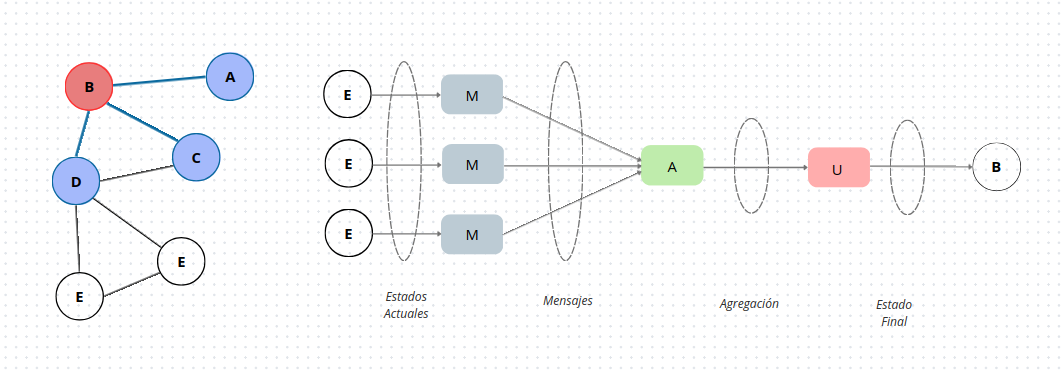
\includegraphics[width=0.7\textwidth]{img/gnn/MPNN.png}        \caption{Flujo de Message passing para un nodo del grafo.}
    \label{fig:pipelineMP}
\end{figure}

\subsection{Graph Convolution Network (GCN)}

Es un tipo específico de MPNN, donde se utilizan convoluciones de grafos para agregar información de los nodos adyacente de un nodo en un grafo. \\

La operación de convolución en el grafo produce la suma normalizada de las características de los nodos vecinos~\ref{ecu:GCN-foormula}. Esta normalización garantiza que la información agregada sea ponderada correctamente, es decir, evitar que un nodo con gran cantidad de vecinos tenga una representación desproporcionada y que luego tenga una influencia mayor en la representación otros nodos en las siguientes capas.\\

La notación de los embeddings de los nodos $h^{(l+1)}_i$ en la capa $l+1$ de la red está dado por: \\



\begin{equation}
    h^{(l+1)}_i = \sigma \left( b^{(l)}_i + \sum_{j \in N(i)} \frac{1}{c_{ji}} h^{(l)}_j W^{(l)} \right)
    \label{ecu:GCN-foormula}
\end{equation}
\\



Donde $\sigma$ se define como la función de activación, $h^{(l)}$ la matriz de características de los nodos en la capa $l$, $W^{(l)}$ la matriz de aprendizaje de pesos, con dimensionalidades dada por el tamaños de atributos entrantes y $c_{ij}$ el termino de normalización.\\


Es así como GCN permite la creación de embeddings para los nodos de un grafo dada la matriz de adyacencia de este, lo que quiere decir que debe conocer el grafo completo para poder realizar la tarea de aprendizaje. Este es un enfoque transductivo, en contraste a otros enfoques inductivos como GraphSAGE.\\

\subsection{Graph Attention Network (GAT)}

Otra variante de MPNN son las Graph Attention Networks (GAT). A diferencia de una Red Neuronal de Convolución, GAT incorpora un mecanismo de atención que permite que cada nodo pondere de forma diferenciada, indicando la importancia de las representaciones de cada vecino para la actualización de las características de un nodo~\cite{GAT}.\\

Los coeficientes se calculan por un mecanismo el cual calcula un puntaje para cada par de nodos. Luego estos puntajes se normalizan por medio de la función softmax (Figura~\ref{fig:calculoGAT}).\\

Así tenemos:\\


\begin{equation}
   z^{(l)}_{i} = W^{(l)} \mathbf{h}^{(l)}_i
   \label{ecu:paso-1-gat}
\end{equation}


\begin{equation}
   e^{(l)}_{ij} = \text{LeakyReLU}(\mathbf{a}^{(l)T}(\mathbf{z}^{(l)}_i || \mathbf{z}^{(l)}_j))
   \label{ecu:paso-2-gat}
\end{equation}


\begin{equation}
   \alpha^{(l)}_{ij} = \frac{e^{(l)}_{ij}}{\sum_{k \in N(i)} \exp(e^{(l)}_{ik})}
   \label{ecu:paso-3-gat}
\end{equation}


\begin{equation}
    h^{(l+1)}_i = \sigma \left(\sum_{j \in N(i)} \alpha^{(l)}_{ij} z^{(l)}_j\right)
    \label{ecu:paso-4-gat}
\end{equation}
\\

Donde~\ref{ecu:paso-1-gat} es la transformación lineal del embedding de la capa anterior $h^{(l)}_i$ con $ W^{(l)}_i$ una matriz de pesos entrenable.\\

La ecuación~\ref{ecu:paso-2-gat} calcula un puntaje de atención entre dos vecinos.  Primero, concatena los embeddings $z$ de dos nodos. Luego realiza el producto punto entre este y una matriz entrenable $a^{(l)}$  y aplica una función LeakyReLU al final.\\

En~\ref{ecu:paso-3-gat} se aplica una función softmax, con el objetivo de normalizar los puntajes de atención en las aristas entrantes de cada nodo.\\

Finalmente, en la ecuación~\ref{ecu:paso-4-gat}, al igual que en GCN, se lleva a cabo la agregación de los nodos vecinos, pero en este caso, se escala por el puntaje de atención. Se utiliza  $\sigma$ como la función de activación que se aplicará a la capa.\\

\begin{figure}[h]
    \centering
    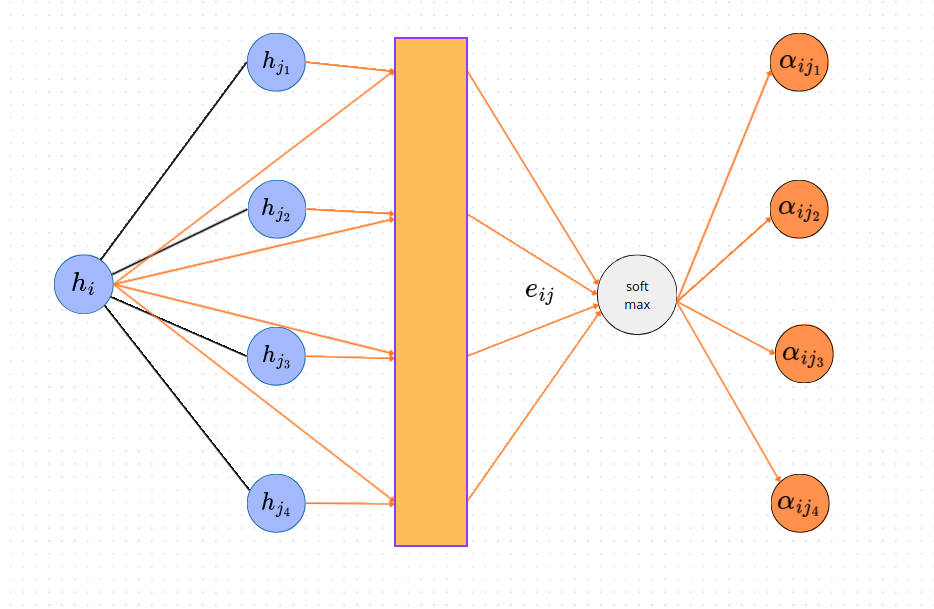
\includegraphics[width=10cm]{img/gnn/GAT.png}
    \caption{Pipeline del mecanismo de cálculo de las ponderaciones para una GAT.}
    \label{fig:calculoGAT}
\end{figure}



\subsection{GraphSAGE (SAmple and aggreGatE)}

Es un framework de aprendizaje inductivo el cual nos permite aprender representaciones de los nodos de un grafo. A diferencia de los enfoques anteriores los cuales son inherentemente transductivos donde se crean las representaciones de los nodos por medio de la recolección de la información de todos sus nodos vecinos, utilizando factorización de matrices, GraphSAGE aprende a crear las representaciones de sus nodos, es decir graphSAGE utiliza las características de nodos de su vecindario y la topología para aprender una función que genera los embeddings en base a un muestreo de nodos vecinos. Ayudado de esta forma a generalizar sobre nodos no vistos naturalmente~\cite{GraphSAGE}. \\

GraphSAGE no necesita de todos sus vecinos durante el entrenamiento para crear una representación del mismo, sino que a través de un subconjunto de estos aprenderá a crear un embedding, que representa su rol local y global en un grafo.\\
 
Que sea inductivo significa que puede crear embeddings para nodos no vistos durante el entrenamiento. Es decir, no necesita conocer todo el grafo ni todos los nodos para crear estas representaciones. 
Este enfoque es útil principalmente a la hora de trabajar con grafos dinámicos, batching/sampling, etc. Representando así a nodos en un vector de baja dimensionalidad y generalizándolo luego para nodos no vistos.\\

El proceso de creación de embeddings para los nodos del grafo está dado por las siguientes ecuaciones:

\begin{equation}
    h^{(l+1)}_{N(i)} = \operatorname{aggregate}\!\left(\left\{ h^l_j \mid \forall j \in N(i)\right\}\right)
    \label{ecu:graphsage-formula-1}
\end{equation}


\begin{equation}
    h^{(l+1)}_i = \sigma\!\left(W \cdot \operatorname{concat}\!\left(h^l_i, h^{(l+1)}_{N(i)}\right)\right)
    \label{ecu:graphsage-formula-2}
\end{equation}

\begin{equation}
    h^{(l+1)}_i = norm(h^{(l+1)}_i)
    \label{ecu:graphsage-formula-3}
\end{equation}

Donde $h^{(l+1)}_{N(i)}$ de~\ref{ecu:graphsage-formula-1} representa las características de los nodos vecinos de un nodo $i$ en la capa $l+1$ el cual, a través de una función de agregación combina estos nodos vecinos. Esta función de agregación puede ser el promedio, suma, lstm u otras.
Luego tenemos $h^{(l+1)}_i$ correspondiente a la concatenación de la representación anterior del nodo $i$ y la de las características de nodos vecinos de la capa $l+1$, correspondiente a lo previamente calculado.
Finalmente tenemos $norm(h^{(l+1)}_i)$ la cual se encarga de normalizar las características del nodo $i$ en la capa $l+1$.\\

La Figura~\ref{fig:graphsage} ilustra el proceso de creación de las representaciones de los nodos. Dado primero 1) por la selección de un número fijo de vecinos de un nodo, 2) luego la agregación y concatenación de las características de estos nodos al nodo destino junto con normalización, y finalmente 3) el paso de predicción y ajuste de valores de los pesos de la red. \\

\begin{figure}[h]
    \centering
    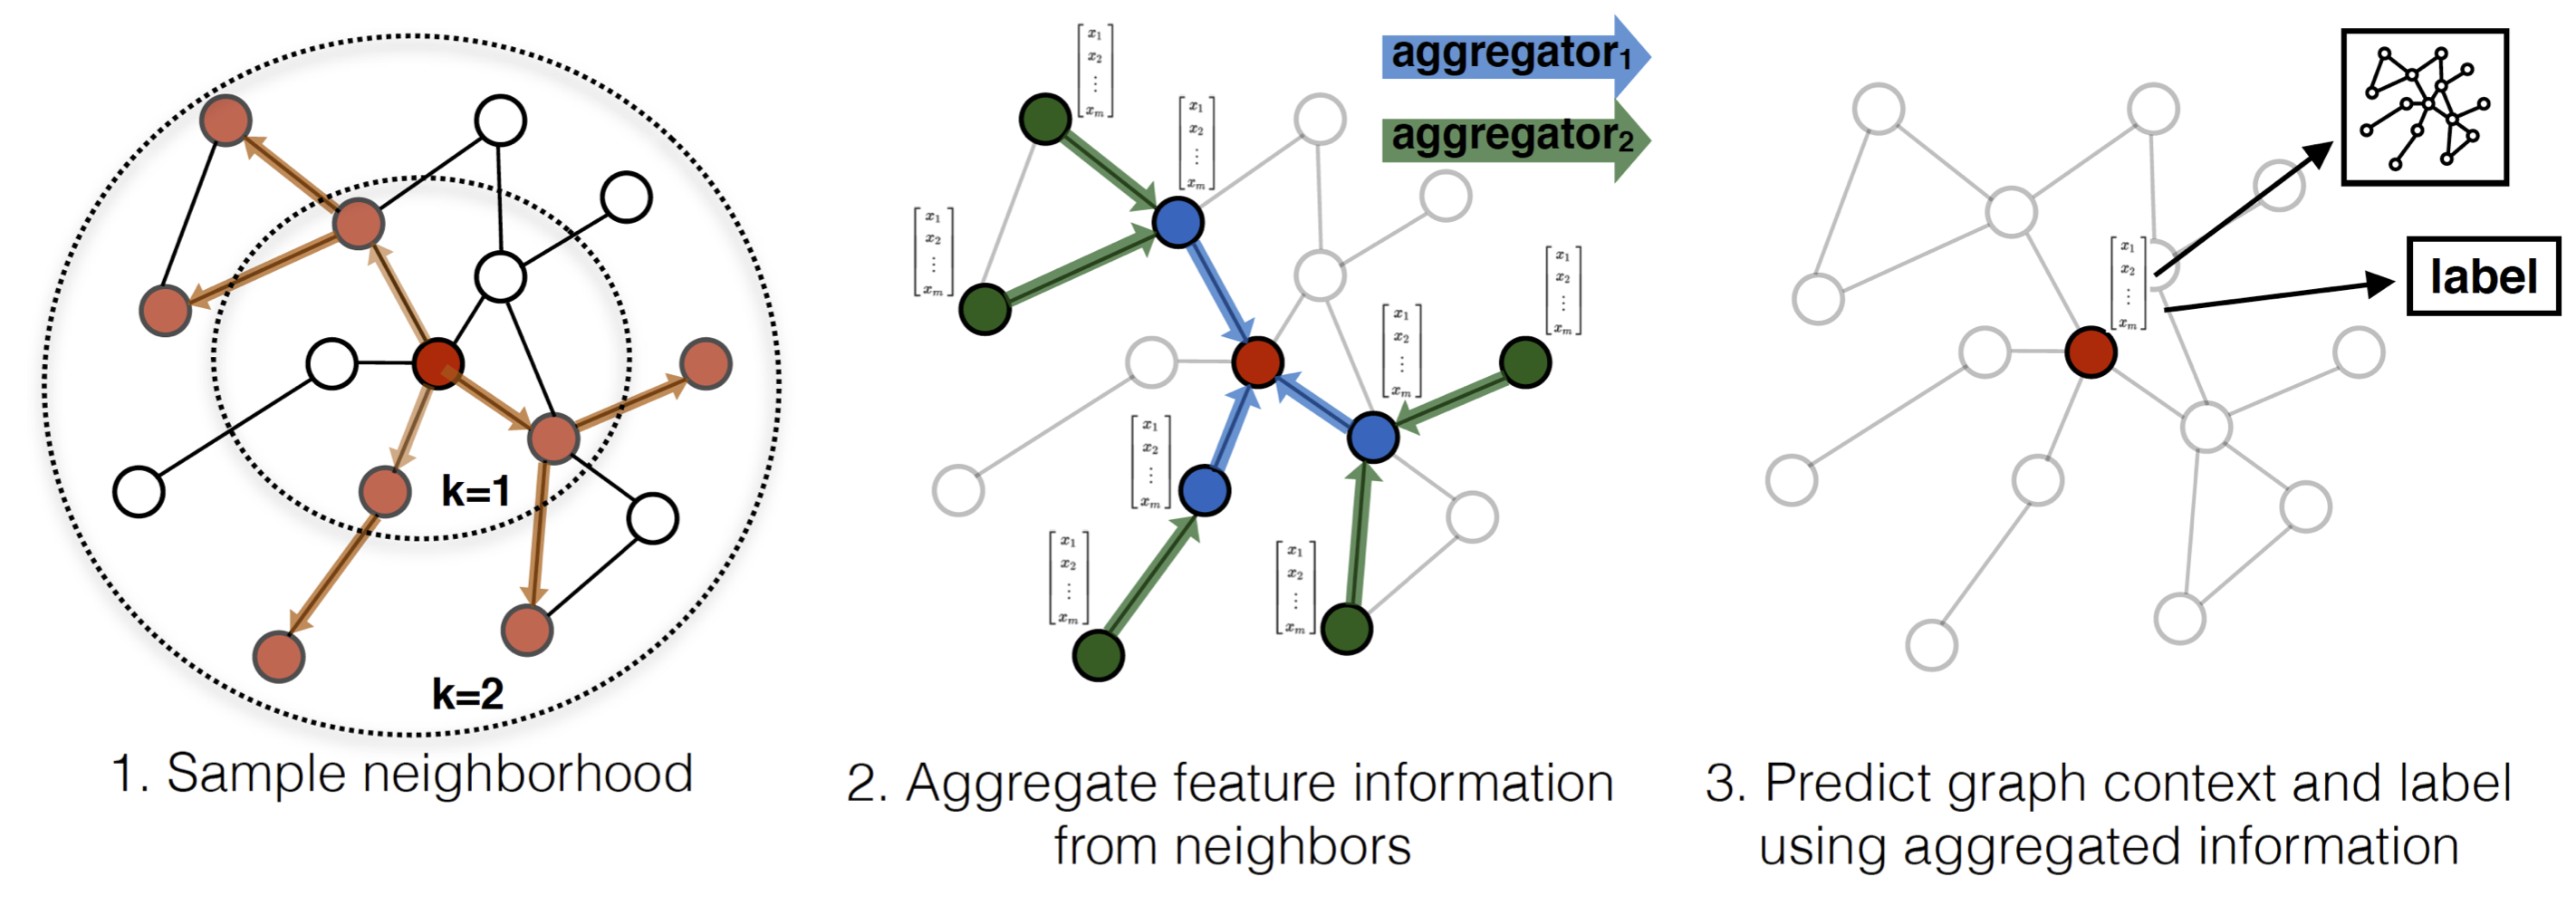
\includegraphics[width=0.7\textwidth]{img/gnn/sample_and_agg.png}
    \caption{Proceso de creación de representaciones de nodos con GraphSAGE.
    Fuente https://snap.stanford.edu/graphsage/}
    \label{fig:graphsage}
\end{figure}


